%                                             -*- coding: utf-8 -*-
% Mindenkinek csak javasolni tudjuk, hogy latex-et használjon.
% Szakdolgozatnál vagy diplománál már egyértelműen kijönnek az
% előnyei a Worddel szemben.  Ennek ellenére ez a sablon messze nem
% tökéletes.  Ha valamit javítanál benne, kérlek, küld vissza, hogy
% hallgatótársaid is profitáljanak belőle.  Köszönöm.

% További nehézséget okoz, hogy a népszerű latex disztribúciók nem
% tartalmazzák a legújabb változatát a magyar.ldf-nek.  A szükséges
% fájlokat a sablon mellé bemásoltuk, de le is tölthetőek innen:
% http://www.math.bme.hu/latex/
%
%
%
\documentclass[11pt,a4paper,oneside]{article}
\usepackage[margin=3cm]{geometry}
% =================================================================
% Magyar nyelvi támogatás
%------------------------
% ###################
% Nyelvváltó parancsok:
%\selectlanguage{english}
%\selectlanguage{magyar}
% rövid angol beszúrás:  \foreignlanguage{english}{some english text}
% határozott névelők generálása ``magyar'' babel-el:
% argumentum+megfelelő határozott nevelő: \az{},\Az{}
% csak a megfelelő határozott nevelő: \az*{}, \Az*{}
% címkék: \aref{}, \aref*{}, képletekhez \aref()
%        \Aref{}, \Aref*{}, képletekhez \Aref()
% oldalak: \apageref{}, \apageref*{}
%        \Apageref{}, \Apageref*{}
% idézetek: \acite, \acite*, \Acite, \Acite*
% ###################
\usepackage[english]{babel} %vegyes nyelvi támogatás a
% magyar helyesírás ellenőrzéshez (ispell) és elválasztáshoz
\selectlanguage{english}

%=================================================================
% direkt ékezetes karakter beírás támogatás
%-------------------------------------------
\usepackage[T1]{fontenc}
\usepackage[utf8]{inputenc}
\usepackage{multirow} 
%================================================================
% Undorító dolog bitmappelt (Type III) betűtípust nézni a PDF-ben
% képernyőn. Az alapértelmezett Computer Modern font LaTex-ben
% bitmappelt, ezért használjunk Times fontot:
\usepackage{times}

%================================================================
% ha ábrát akarunk beemelni, akkor használjuk a graphicx/graphics
% csomagot és az \includegraphics[width=<width>]{abra.pdf} parancsot
\usepackage{graphicx} %for graphics
%kepek helye a gyokerhez(ehhez a file-hoz kepest) kepest
\graphicspath{{./figs/}}

%================================================================
% Kötelezően használjuk a hyperref csomagot, mert ezzel többek között 
%  kultúrált hyperlinkelt PDF-et lehet csinálni az alábbi
%  variációkban, különféle hyperref backend-ekkel:
%  pdflatex,dvipdfm,ps2pdf
% tapsztalataim szerint a MikTeX (Win32) a 'dvipdfm' konverzióval
% optimális  míg a teTeX (Linux/Solaris) jobb szereti a 'dvips' módszert
%------------------------------------
% pontosan egyet kommentezzünk be!!!!!!!
% értelemszerűen backend függően generáljunk dvi-ból PDF-et!!!
%------------------------------------
% A hyperref csomag az utolsó beolvasott csomag legyen, kivéve néhány
% problémás csomagot, pl. algorithm
%-----------
% ########################### FONTOS ###########################
% A hyperref hibásan működik a babel csomag 'magyar.ldf' fájljának
% 1.5-ös verziójánál korábbi változatával. 2004. februárjában a MikTeX
% és teTex disztribúciók még csak a v.1.4 verziót tartalmazták! A fájl
% aktuális verziója a BME Matematikai intézet LaTeX honlapjáról
% elérhető: http://www.math.bme.hu/latex/ 
% A lusták kedvéért a jelen sablon mellé is mellékelem:
% magyarlatex_0.01-2.tar.gz 
% ########################### FONTOS ###########################
%-----------
\PassOptionsToPackage{hyphens}{url}\usepackage[colorlinks=true]{hyperref}
\def\equationautorefname~#1\null{Equation (#1)\null}
\def\figureautorefname~#1\null{Figure (#1)\null}
\def\tableautorefname~#1\null{Table (#1)\null}

%%%%%%%%%%%%%%%%%%%%%%%%%%%%%%%%%%%%%%%%%%%%%%%%%%%%%%%%%%%%%%%%%%%
% Itt kezdődik maga a dokumentum
%%%%%%%%%%%%%%%%%%%%%%%%%%%%%%%%%%%%%%%%%%%%%%%%%%%%%%%%%%%%%%%%%%
\begin{document}
%%%%%%%%%%%%%%%%%%%%%%%%%%%%%%%%%%%%%%%%%%%%%%%%%%%%%%%%%%%%%%%%%%%
% Ezt ne piszkáld!!!!
%%%%%%%%%%%%%%%%%%%%%%%%%%%%%%%%%%%%%%%%%%%%%%%%%%%%%%%%%%%%%%%%%%%
\pagestyle{myheadings} % legyen fejléc 

\newcommand{\semesterprojecttitle}{
  \begin{center}
    \huge{\textbf{Project Laboratory Report}}
    
    \smallskip
    \small{Department of Telecommunications and Media Informatics}
  \end{center}
  \bigskip
} 

% Argumentumok: #1=Név, #2=Neptunkód, #3=szakirány, #4=email, #5 konzulens-1, #6 konzulens-1-email, #7 konzulens-2, #8 konzulens-2-email
\newcommand{\semesterprojectauthor}[6]{

\begin{center}
  \begin{tabular}{ l c }
  Author:         & \textbf{#1}  \\
  Neptun:         & \textbf{\texttt{#2}}  \\
  Specialization: & \textbf{#3}  \\
  E-mail address: & \href{mailto:#4}{\textbf{#4}}  \\
  Supervisor:     & \textbf{#5}  \\
  E-mail addres:  & \href{mailto:#6}{\textbf{#6}} \\
  
  \end{tabular}
\end{center}
\bigskip

}

% % Argumentumok: #1=Név, #2=email
% \newcommand{\konzulens}[2]{
%   \noindent\textbf{Konzulens:} #1 
%   \newline\emph{Email cím:}\/ \href{mailto:#2}{#2}
%   \newline
% 
% }

% Argumentumok: #1=Tanév (xxxx/xx alakban, #2=félév (pont nélkül)
\newcommand{\semester}[2]{
  \large\textbf{#1 #2. semester}
}

% Argumentumok: #1=téma címe 
\newcommand{\tasktitle}[1]{
  \begin{center}
    \LARGE\textbf{Title: #1}
    \bigskip
  \end{center}
}

% Argumentumok: #1=téma részletei 
\newcommand{\taskdescription}[1]{
\begin{center}
  \Large\textbf{Task} 
\end{center}
#1
\newline
\bigskip
}

% A fejezetek közé beágyazott irod.jegyzék
\def\references#1{\renewcommand{%
\baselinestretch}{1}\list
 {\small [\arabic{enumi}]}{\settowidth\labelwidth{[#1]}\leftmargin\labelwidth
 \advance\leftmargin\labelsep
 \usecounter{enumi}}
 \def\newblock{\small \hskip .11em plus .33em minus .07em}
 \sloppy\clubpenalty4000\widowpenalty4000
 \sfcode`\.=1000\relax}
\let\endreferences=\endlist%


%%% Local Variables: 
%%% mode: latex
%%% TeX-master: "template"
%%% End: 
 % Ez kell!!!
\markright{Márton Torner (OZFKFP)} % egyoldalas fejléc!!!

%--------------------------------------------------------------------
% fedlap
%--------------------------------------------------------------------
\begin{titlepage}
%bme logo 
 \begin{figure}[h]
    \centering
      
\includegraphics[width=12cm]{bme_logo}
  \label{fig:bme_logo}
  \end{figure}
  \thispagestyle{empty}
  %cím generálás
  \semesterprojecttitle
 
  %\author argumentumok: #1=Név, #2=Neptunkód, #3=szakirány, #4=email,#5 konzulens-1, #6 konzulens-1-email, #7 konzulens-2, #8 konzulens-2-email
  \semesterprojectauthor{Márton Torner}{OZFKFP}{Infocommunication (HIT)}{torner.marton@gmail.com}{Bálint Gyires-Tóth, PhD}{toth.b@tmit.bme.hu}
 
 
%\tasktitle argumentuma a task rövid, 1 soros címe
  \tasktitle{Financial time series modeling and forecasting with deep neural networks} 

  %\taskdescription argumentuma a task 1-2 bekezdésnyi ismertetése
  \taskdescription{The task is to collect limit order book data from a chosen crypto exchange, 
  analyze and process the gathered records and to develop a neural network based solution to predict 
  the direction of the price movement of the asset-pairs.
  
  In this work level 100 data (limit order book, depth: 100) is used from Kraken crypto exchange. The live order flow 
  is queried with the help of the provided API and saved on a local storage. The aim is to create a Deep Learning 
  powered system which can predict the price movement direction from the given history. The first approaches are 
  models based on autoregressive solutions (logistic regression and random forest regression) and then I try to use a 
  deep neural network as the model.
  
  In the future this work can be used as a base for creating a complex system for algorithmic trading.}

  %\semester argumentumok:
  % #1=Tanév (xxxx/xx alakban), #2=félév (pont nélkül!)
  \begin{center}
    \semester{2018/19}{II}
  \end{center}
  
\end{titlepage} 

%==================================================================
\begin{center}
  \section{Theory and previous works}
  \label{sec:theory_prev}
\end{center}
% A munka  előzményei és kiindulási állapota
% \newpage
\subsection{Introduction}
\label{sec:introduction}

The computerization of financial markets and the availability of the electronic records of different stock exchanges 
like transactions, order flow and limit order books provide us a great opportunity to analyze and model the dynamics of 
these markets. Over the last years a huge number of studies have been done on this field which can serve as a good base 
for further studies.

With the computerization also came the rapid acceleration of the trading on these financial markets and big companies 
started to use algorithmic solutions to steal a march on their rivals and gain some higher profits.

The quick development that the field of Deep Learning had in the last decade and the impressive number of successful 
researches conducted on the topic of time series forecasting opened the door to change the traditional mathematical 
algorithms with a neural network based solutions. Price forecasting is just a step leading to more complex systems 
which use the predictions as inputs to deliver a trading strategy with the help of machine learning 
(reinforcement learning).

These solutions could change the role of financial specialists in the future.

\subsection{Theoretical summary}
\label{sec:theoretical_summary}

  \subsubsection{Price formation mechanism}
  \label{sec:price_formation_mechanism}
  
  The market price per share of stock (“share price”) is the amount of money an investor is willing to pay to own 
  a company's single stock. The ‘price formation mechanism’ - given in \autoref{eq:1} - is a map which tries to 
  represent the relation between market price and different variables affecting it, e.g. price history, order flow, 
  news about the companies or the market etc.

  \begin{equation}
    Price(t+\Delta t) = F(Price history(0...t), Order Flow(0...t), Other Info) = F(X_{t}, \epsilon_{t})
    \label{eq:1}
  \end{equation}


  \begin{center}
    \begin{tabular}{l l}
      $X_{t}$: & set of state variables (e.g. order flow, volatility, price, etc.) \\
      $\epsilon_{t}$: & random noise (represents the arrival of new, unknown information) \\
      $\Delta t$: & time resoution
    \end{tabular}
  \end{center}

  \bigskip

  It is shown that this relation is universal (not asset-specific) and stationary (stable across time, even at 
  out-of-sample predictions) ~\cite{univ}. These two features give us the opportunity to use all collected data points 
  to design and train a universal model which can make predictions for all asset-pairs valid even in the future.

  \subsubsection{Limit Order Book}
  \label{sec:limit_order_book}
  
  In this work limit order book data is used as the input so this section tries to provide a short overview what it is 
  and how it works. On stock exchanges we want to buy shares or sell the ones we hold and to accomplish this we place 
  orders of which the LOB consists. There are more special types of orders but in this work only limit orders are used. 
  They remain in the LOB until being executed or cancelled.
  
  The LOB has two sides, the ask and the bid side, shown on \autoref{fig:1}. The ask side represents the sell orders 
  (willing to sell the given amount at the given price) and the bid side the buy orders (willing to buy the given amount 
  at the given price).

  \begin{figure}[tbh]
    \centering
    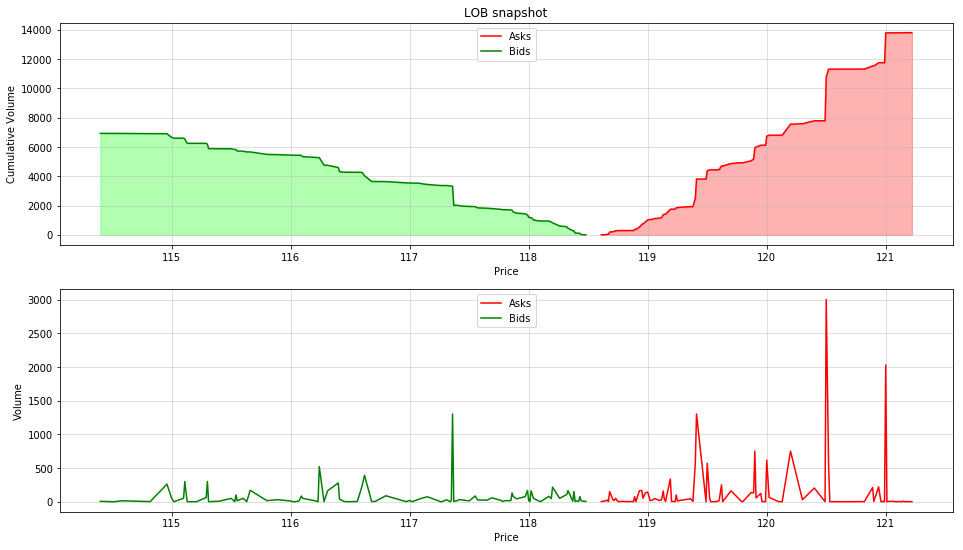
\includegraphics[width=\textwidth]{lob_snapshot.png}
    \caption{Limit Order Book snapshot (ETH\_EUR). Bottom: Volume at each price level. Top: Cumulative volume at price levels.}
    \label{fig:1}
  \end{figure}

  A tick is the measure of the minimum upward or downward movement in a price of a security this means the price levels 
  in the LOB must be the multiples of this value (so order prices can not differ less than this). The best ask price is 
  the lowest sell order and the best bid price is the highest buy order. These are the prices at which the given number 
  of shares can be bought or sold. The difference between best ask and bid price is called the spread and their average 
  is the mid-price. The weighted average mid-price (WAMP) and volume weighted average price (VWAP) can be calculated as 
  given in \autoref{eq:2} and \autoref{eq:3}. The depth of the book is used in this paper as the number of best orders 
  on each side (so depth=100 means the top 100 lowest priced ask- and the top 100 highest priced bid orders).

  \begin{equation}
    WAMP = \frac{p_{best}^{bid} * v_{best}^{ask} + p_{best}^{ask} * v_{best}^{bid}}{v_{best}^{bid} + v_{best}^{ask}}
    \label{eq:2}
  \end{equation}

  \begin{equation}
    VWAP = \frac{(\sum_{i=1}^{depth} (p_i^b * v_i^b))*v^a + (\sum_{i=1}^{depth} (p_i^a * v_i^a))*v^b}{v^a + v^b}
    \label{eq:3}
  \end{equation}

  \begin{center}
    \begin{tabular}{l l}
      $p$: & price \\
      $v$: & volume (without lower index = sum over side) \\
      $b$: & bid \\
      $a$: & ask
    \end{tabular}
  \end{center}

  Orders are submitted and cancelled continuously which means that the updates arrive in a very high frequency 
  (millisecond) and it is also easy to see that consuming the order flow of stock exchanges leads to Terabytes of data. 
  At crypto exchanges order manipulation is a big problem to be faced at filtering the collected data. So, to process a 
  live order book we have to deal with various problems [TODO link ide a crawler szekcióhoz].

  \subsubsection{Deep Learning}
  \label{sec:deep_learning}

  Deep Learning models are deep neural networks (an example can be seen on \autoref{fig:2}) trained on large datasets to 
  uncover complex non-linear relations between the (high-dimensional) inputs and outputs. This can be simplified as it 
  represents a functional relation like y = f(x) where y is the output and x is a (high-dimensional) input vector.

  \begin{figure}[tbh]
    \centering
    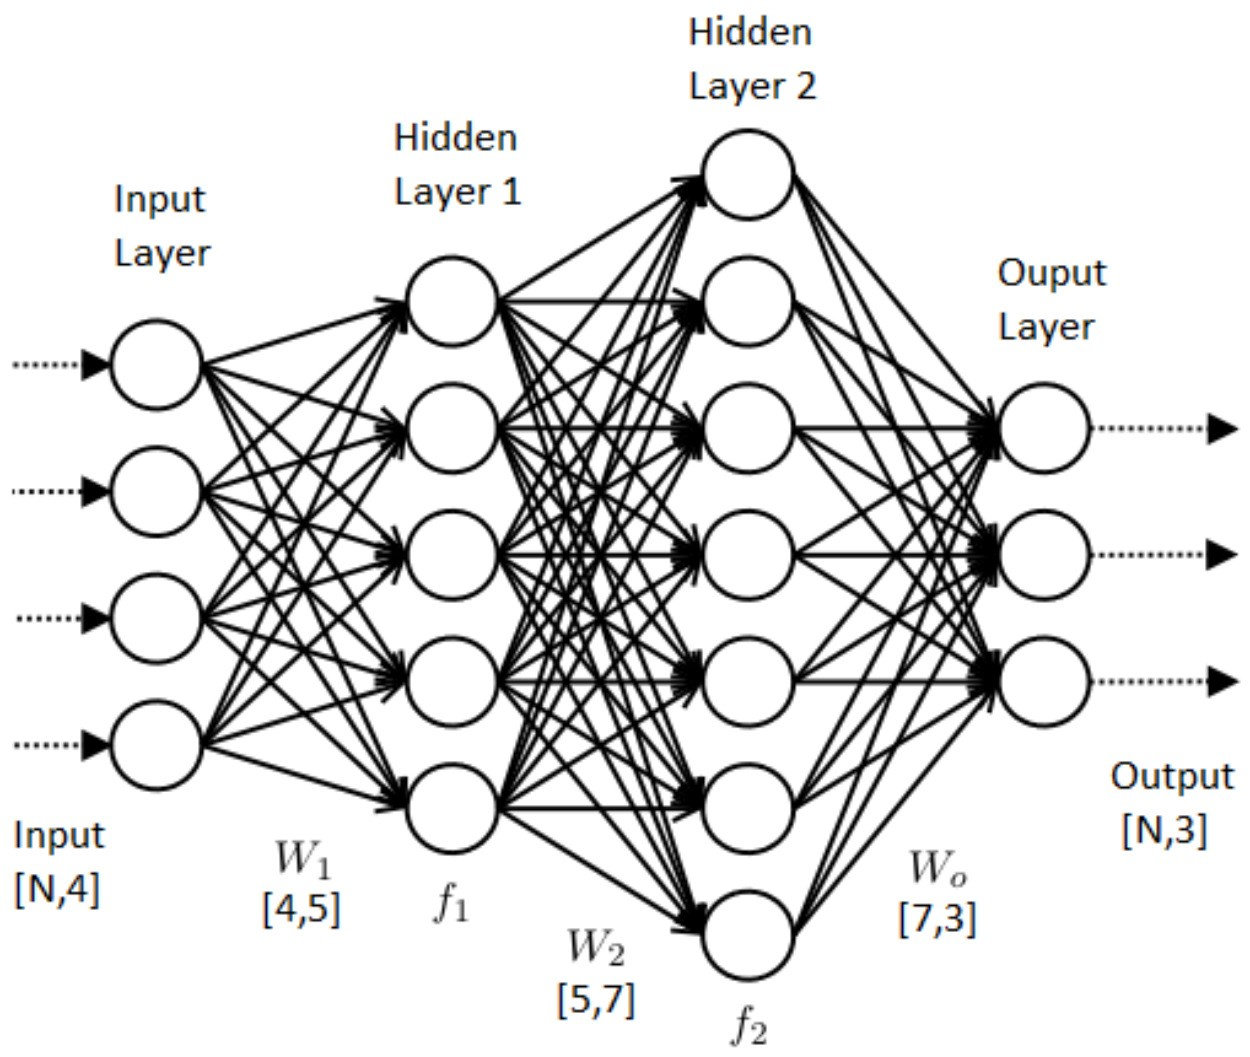
\includegraphics[width=8cm]{mlp.png}
    \caption{Simple multilayer perceptron.}
    \label{fig:2}
  \end{figure}

  The network iterates the input data through its hidden layer(s) (basically weighted sums are calculated followed by 
  so called ‘activation’ functions). In supervised approaches the weights are modified in the backpropagation process 
  in which a regularized cost function – reflecting the discrepancy between the inputs and the desired output – is tried 
  to be optimized. Depending on the input and output dimensionality and the design of the network it can have millions 
  of parameters which makes these calculations computationally expensive. This problem made the development of this 
  field a standstill until the rapid spread and improvement of GPUs started providing a huge advancement in 
  calculations.

  \subsubsection{Convolutional Networks}
  \label{sec:conv_nets}

  A class of deep neural networks are convolutional neural networks (CNN). The main design is the same as any other 
  networks (input, hidden layers, output). General CNNs use a set of convolutional layers followed by fully-connected 
  layers (all neurons in a layer are connected to every neuron in the preceding and following layers as seen on 
  \autoref{fig:2}) as hidden layers. Convolutional layers are used for representing small or high features in the data 
  with applying a convolutional operation to their input. It uses filters which are parts of the data with the same or 
  less dimension than the input. Using $k$ filters $k$ feature maps are generated.
  
  Attention is a mechanism which can be added to reach better results with the cost of more computational expenses 
  ~\cite{attention}. At a high-level attention can be described as giving the network the ability to learn which parts 
  are more important to focus on. It is commonly and successfully used at natural language processing tasks.

  \subsubsection{Generative Adversarial Networks}
  \label{sec:gans}

  Generative adversarial networks (GAN) are deep neural architectures comprised of a generator and a discriminator 
  network (\autoref{fig:3}), introduced by Goodfellow et al. ~\cite{gan}. These two networks contest against each other 
  in the following way. The aim of the generator is to produce data indistinguishable of the real data and the 
  discriminator tries to classify whether its input was real data or fake, generated by the opposing network. The losses 
  of the networks are propagated back combined making both networks’ reward depending on both of their performance. This 
  means if the generator lacks competence the discriminator’s work will be easy thus the system will be incompatible of 
  solving the problem. The design and training of GANs is a complex task.

  \begin{figure}[tbh]
    \centering
    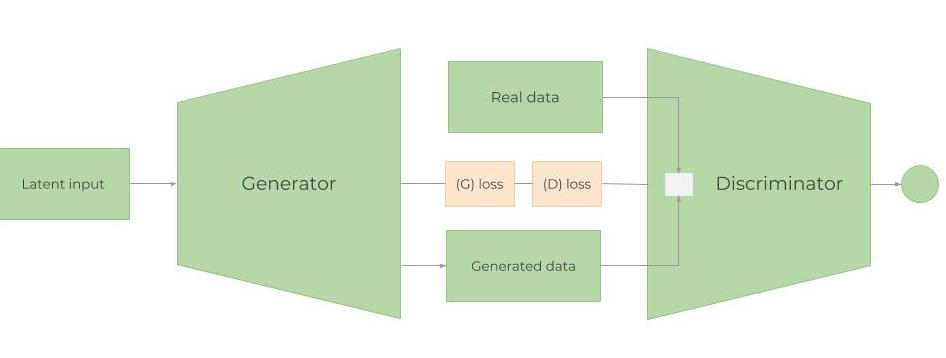
\includegraphics[width=12cm]{gan.jpg}
    \caption{GAN architecture example.}
    \label{fig:3}
  \end{figure}

\subsection{Starting point, previous works on this project}
\label{sec:prev_works}

At the start of the project I was no preceding work given and did not make any research on this topic before.

I started learning the theory of Deep Learning as part of the university course VITMAV45 and gained a well based 
knowledge on the subject to start with.

\newpage
%==================================================================
\begin{center}
  \section{Own work on project}
  \label{sec:work}
\end{center}

\subsection{Data}
\label{sec:data}

The project's first task was to find or collect a database to work with. On financial field the big and high frequency 
raw datasets which are precise enough can cost a lot of money (3000 USD+). There was no funding available so I collected 
my own raw data from Kraken (\url{www.kraken.com}) which is a US based cryptocurrency exchange. Kraken gives the 
opportunity to access live order book (and of course other) data through a REST- and a Websocket based API. 

In the training and evaluation process only ETH\_EUR \footnote{Ethereum - Euro: Ethereum is an open-source, public, 
blockchain-based distributed computing platform and operating system featuring smart contract (scripting) functionality. 
- \textit{Wikipedia} } snapshots are used but for further research on universality and stationarity ~\cite{univ} I save 
25 asset-pair's data in aggregate. For each 1 snapshot is querried every minute through REST API calls and the 
real-time order flow is recorded through the previosly mentioned Websocket API. 

The saved data is stored in CSV file format, \autoref{table:1} and \autoref{table:2} show the structure. Every 
asset-pair is saved to a separate folder and at the end of each day all buffer files (updates and snapshots) are 
compressed and saved into a separate file this way saving space and ensuring that the unexpected corruption of a file 
causes minimal data loss. The saving method also makes paralell datapreparation on multiple CPUs possible. 
The dataset contains entries from 15th March 2019.

\begin{table}[tbh]
  \centering
  \begin{tabular}{|l|l|}
    \hline
    Field              & Description \\
    \hline
    L1 Ask Price       & The price of the ask order at 1st level (best ask) \\
    \hline
    L1 Ask Volume      & The volume of the ask order at 1st level \\
    \hline
    L1 Ask Timestamp   & The last modification time of the ask order at 1st level \\
    \hline
    ... \\
    \hline
    L100 Ask Price     & The price of the ask order at 100th level \\
    \hline
    L100 Ask Volume    & The volume of the ask order at 100th level \\
    \hline
    L100 Ask Timestamp & The last modification time of the ask order at 100th level \\
    \hline
    L1 Bid Price       & The price of the bid order at 1st level (best bid) \\
    \hline
    L1 Bid Volume      & The volume of the bid order at 1st level \\
    \hline
    L1 Bid Timestamp   & The last modification time of the bid order at 1st level \\
    \hline
    ... \\
    \hline
    L100 Bid Price     & The price of the bid order at 100th level \\
    \hline
    L100 Bid Volume    & The volume of the bid order at 100th level \\
    \hline
    L100 Bid Timestamp & The last modification time of the bid order at 100th level \\
    \hline
    Timestamp          & The timestamp of the snapshot \\
    \hline
  \end{tabular}
  \caption{One snapshot (one row in snapshot files).}
  \label{table:1}
\end{table}

\begin{table}[tbh]
  \centering
  \begin{tabular}{|l|l|}
    \hline
    Field       & Description \\
    \hline
    AskOrBid    & The update type: 0 = ask, 1 = bid \\
    \hline
    Price       & The price of the order \\
    \hline
    Volume      & The volume of the order (0 means that the level is deleted)\\
    \hline
    Timestamp   & The last modification time \\
    \hline
  \end{tabular}
  \caption{One update (one row in update files).}
  \label{table:2}
\end{table}

  \subsubsection{Data preparation}


\subsection{Summary}
\label{sec:summary}

A félévi munka során elért új eredmények ismételt, vázlatos, tömör
Ebben a részben az adott félévre vonatkozó, az \emph{Önálló
  laboratórium tárgy keretében elvégzett munka során} elért
\textbf{új} eredmények ismételt, vázlatos, \textbf{tömör}
összefoglalását várjuk, lehetőleg nem felsorolásként.  Itt még egyszer
ki lehet térni a leglényegesebb eredményekre, valamint a félév során
felmerülő nehézségekre, de meg lehet említeni a továbbfejlesztési
irányokat, lehetőségeket is.

Ezt a részt tagolható a következő pontok megválaszolásával:
\begin{itemize}
\item Mi volt az \textbf{aktuális kérdés}, probléma, amivel a félév
  során foglalkoztál?
\item Mi a dolgozat \textbf{célja}, miért érdekes egyáltalán ezzel a
  problémával foglalkozni?
\item Milyen \textbf{módszereket} használtál a probléma megoldása
  érdekében?
\item Mik a legfontosabb \textbf{eredmények}?
\item Milyen \textbf{következtetéseket} lehet levonni?

\end{itemize}

Ha valaki elolvassa ezt a részt, képet kell kapnia az egész
dolgozatról.  Ne legyen az absztrakt szó szerinti ismétlése.

Fontos, hogy az itt megadott sablontól el lehet térni, használata nem
kötelező, csak segítséget jelenthet, viszont a fedőlap lehetőleg
maradjon ugyanez és tartalmilag egyezzen meg a sablon irányelveivel. A
beszámoló felépítésében nem érdemes eltérni a \emph{Bevezető --
  Féléves munka és eredmények bemutatása -- Összefoglaló} hármastól.

\newpage
%==================================================================
\section{References}
\label{sec:irod-es-csatl}

\begin{references}{9}
\label{sec:tanulm-irod-jegyz}

\bibitem{univ} Justin Sirignano and Rama Cont (2018). \emph{
\href{https://arxiv.org/abs/1803.06917.pdf}{Universal features of price formation in financial markets: perspectives from Deep Learning}}

\bibitem{attention} \emph{\href{https://medium.com/syncedreview/a-brief-overview-of-attention-mechanism-13c578ba9129}{A Brief Overview of Attention Mechanism}}

\bibitem{gan} Ian J. Goodfellow, Jean Pouget-Abadie, Mehdi Mirza, Bing Xu, David Warde-Farley, Sherjil Ozair, Aaron Courville, Yoshua Bengio (2014). \emph{
\href{http://papers.nips.cc/paper/5423-generative-adversarial-nets.pdf}{Generative Adversarial Nets}}

\bibitem{boris} \emph{\href{https://github.com/borisbanushev/stockpredictionai}{Using the latest advancements in AI to predict stock market movements}}

\bibitem{deeplob} Zihao Zhang, Stefan Zohren, and Stephen Roberts (2019). \emph{
\href{https://arxiv.org/abs/1803.06917.pdf}{DeepLOB: Deep Convolutional Neural Networks for Limit Order Books}}

\end{references}

%==================================================================
\subsection{Source code}
\label{sec:source_code}

The whole project's source code (except the crawler's) can be found on GitHub: \\ 
\url{https://github.com/tornermarton/SemesterProject} \\
On some topics a deeper insight/longer explanation can be found in the Markdown files under the docs folder. \\
Most of the images used here can be found in the Jupyter Notebooks which are publicated also in this repository. \\

\vspace{5mm}
\noindent{The following library served as a base for the crawler:} \\
\url{https://github.com/krakenfx/kraken-wsclient-py} 

\end{document} 

%%% Local Variables: 
%%% mode: latex 
%%% TeX-master: t 
%%% End:

